\section{PCB Technologies}

	\subsection{Basic Board Materials}
		\begin{itemize}
			\setlength{\itemsep}{0pt}
			\item \textbf{FR-4 Laminates}
			\setlength{\itemsep}{-5pt}
			\item[] Layer of woven glass cloth impregnated with epoxy-resin (Epoxidharz)
			\item[] Yellow translucent (green comes from solder mask)
			\setlength{\itemsep}{0pt}
			\item \textbf{FR-2 Laminates}
			\setlength{\itemsep}{-5pt}
			\item[] Layer of cellulose paper (Kraftpapier) impregnated with phenolic resin (Phenolharz)
			\item[] Cheaper than FR-4
			\item[] Holes/Profile by punching (stanzen)
			\item[] Opaque brown 
			\item[] For cheap consumer electronics 
		\end{itemize}
		
	\subsection{Laminate Production}
		\begin{figure}[h]
			\centering
			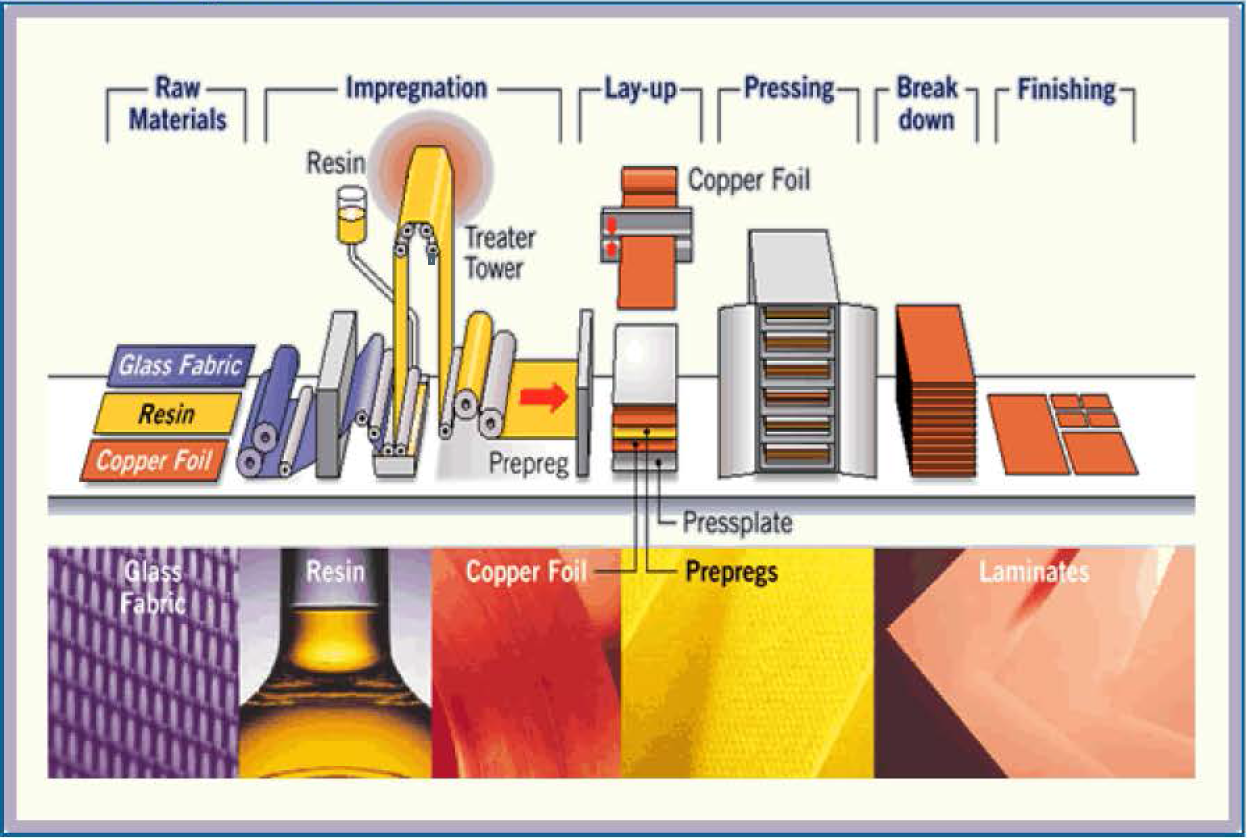
\includegraphics[width=0.75\textwidth]{images/LaminateProduction.png}
			\caption{Laminate Production}
			\label{Fig:LaminateProduction}
		\end{figure}
			
	\subsection{Laminate Production}
	Different resins lead to different characteristics (e.g. viscosity increase, flame retarding) of the laminate. The different resin types are listed below: 
		\begin{figure}[h]
			\centering
			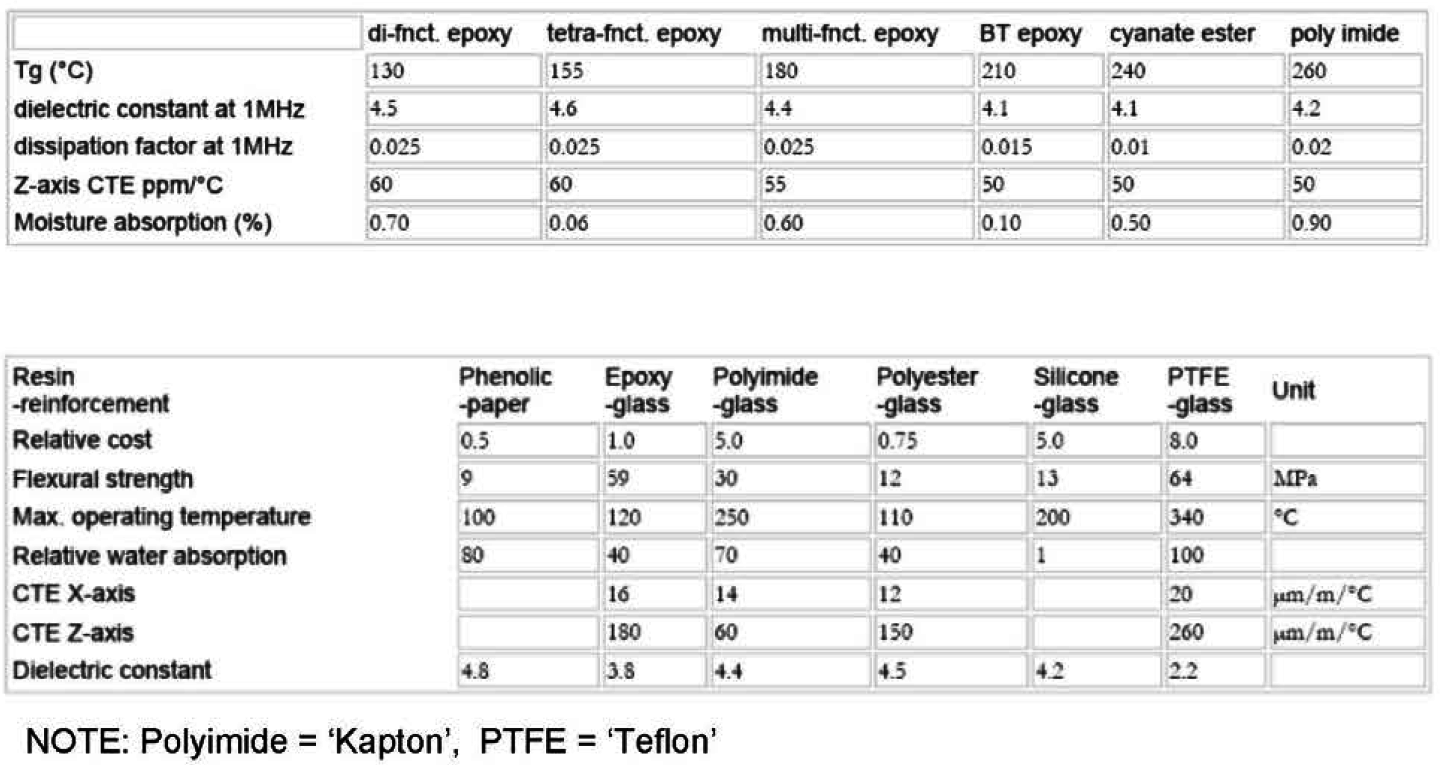
\includegraphics[width=0.75\textwidth]{images/ResinTypes.png}
			\caption{Different Resin Types with their Properties}
			\label{Fig:ResinTypes}
		\end{figure}
	\subsection{Other Reinforcement (Verstärkungs-) Material}
		\begin{itemize}
			\setlength{\itemsep}{0pt}
			\item \textbf{Chopped-Strand Matte (Strand = Faden)}
			\setlength{\itemsep}{-5pt}
			\item[] A Matte reinforcement improves homogeneity, since there is more random orientation of the reinforcement material. Chopped-Strand Matte is the most common type, it consists of chopped fibres with a length of 25 to 150 mm, which are distributed evenly in the resin. 
			\setlength{\itemsep}{0pt}
			\item \textbf{Continuous Strand}
			\setlength{\itemsep}{-5pt}
			\item[] Continuous strands of fibre are distributed in a random spiral orientation. This 'non-woven' structure is used for aramid fibre reinforcement. Advantages: Lighter epoxy laminate, lower CTE (Coefficient of Thermal Expansion), lower dielectric constant, easier to process with laser ablation (Abtragung), for very tiny holes etc. 
		\end{itemize}	
	\subsection{Qualitative Comparison of Laminates}	
		\begin{figure}[h]
			\centering
			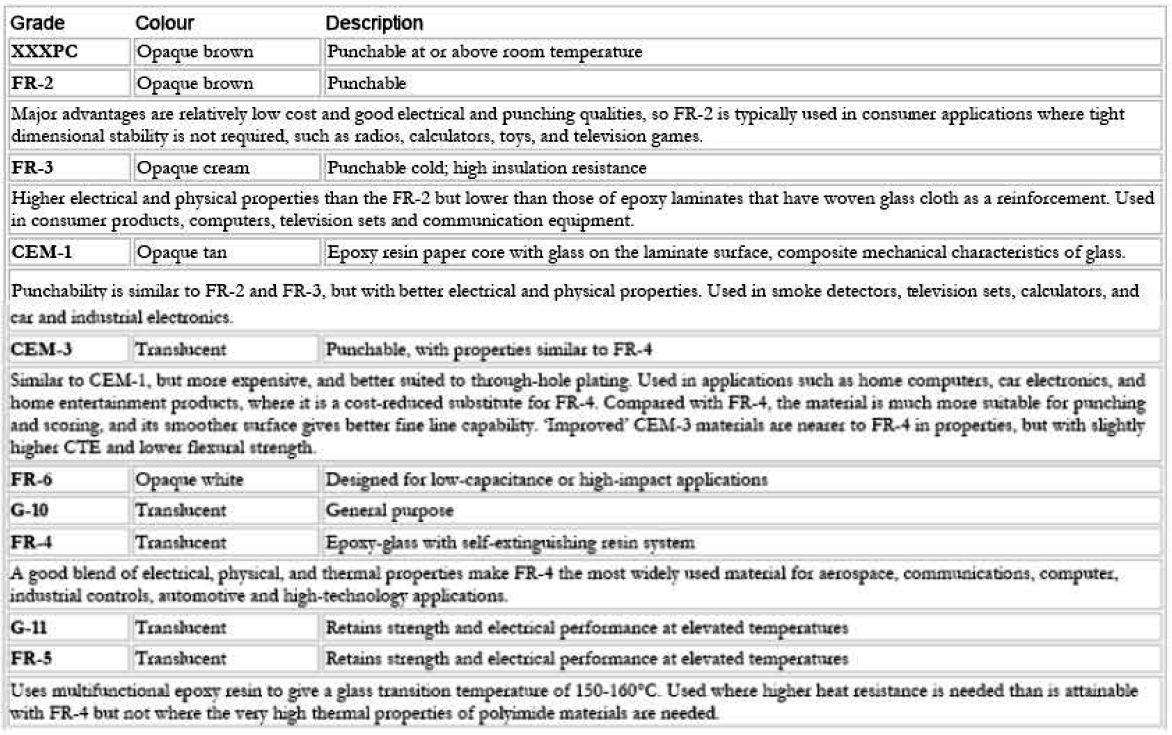
\includegraphics[width=0.75\textwidth]{images/LaminateComparison.png}
			\caption{Laminate Comparison}
			\label{Fig:LaminateComparison}
		\end{figure}		
			
	\subsection{Thermal Expansion - CTE}
		The thermal expansion coefficient CTE is given by: 
		\begin{equation}
			\alpha = \frac{dl}{l\cdot dT} \qquad[K^{-1}]
		\end{equation}
		with 
		\begin{itemize}
			\setlength{\itemsep}{-5pt}
			\item[] \makebox[1.5em][l]{$dl$} = Change in length of the material in the direction being measured
			\item[] \makebox[1.5em][l]{$l$} = Overall length of material in the direction being measured
			\item[] \makebox[1.5em][l]{$dT$} = Change in temperature over which $dl$ is measured
		\end{itemize}
		
		\begin{table}[h!]
			\centering
			\begin{tabular}{|l|c|}
				\hline
					\textbf{Material} & \textbf{CTE (ppm/$^\circ$C)}\\
				\hline
				\hline
					Silicon & 3.2 \\
				\hline
					Alumina & 6-7 \\
				\hline
					Copper & 16.7\\
				\hline
					Tin-Lead Solder & 27 \\
				\hline
					E-Glass & 54 \\
				\hline
					S-Glass & 16 \\
				\hline
					Epoxy Resins & 15-100 \\
				\hline	
					Silicone Resins & 30-300\\	
				 \hline
			\end{tabular}
			\caption{Typical CTE values}
			\label{Tab:CTEValues}
		\end{table}
		The CTE is often not the same for all axes (not isotropic). The CTE for PCB laminates differs from the XY plane to the Z plane. The CTE is rarely linear. 
	\subsection{Glass Transition Temperature - $T_g$}
		TMA = Thermo-Mechanical Analysis defines the glass transition in terms of the change in the coefficient of thermal expansion (CTE) as the polymer goes from glass to rubber state with the associated change in free molecular volume. \\
		Benefits of high $T_g$:
		\begin{itemize}
			\setlength{\itemsep}{-5pt}
			\item The higher the $T_g$ the lower the total amount of Z-direction movement $\rightarrow$ Reduced stress on the PCB during heating processes. 
			\item The higher the $T_g$ the less likely will pads and lines detach from the PCB surface. 
			\item The higher the $T_g$ the less likely will the resin separate from the glass weave due to differential expansion of glass and resin. 
			\item The higher the $T_g$ the better will be the long term thermal stability of a material. 
		\end{itemize}
			
	\subsection{Surface Resistivity}
		\begin{figure}[h]
			\centering
			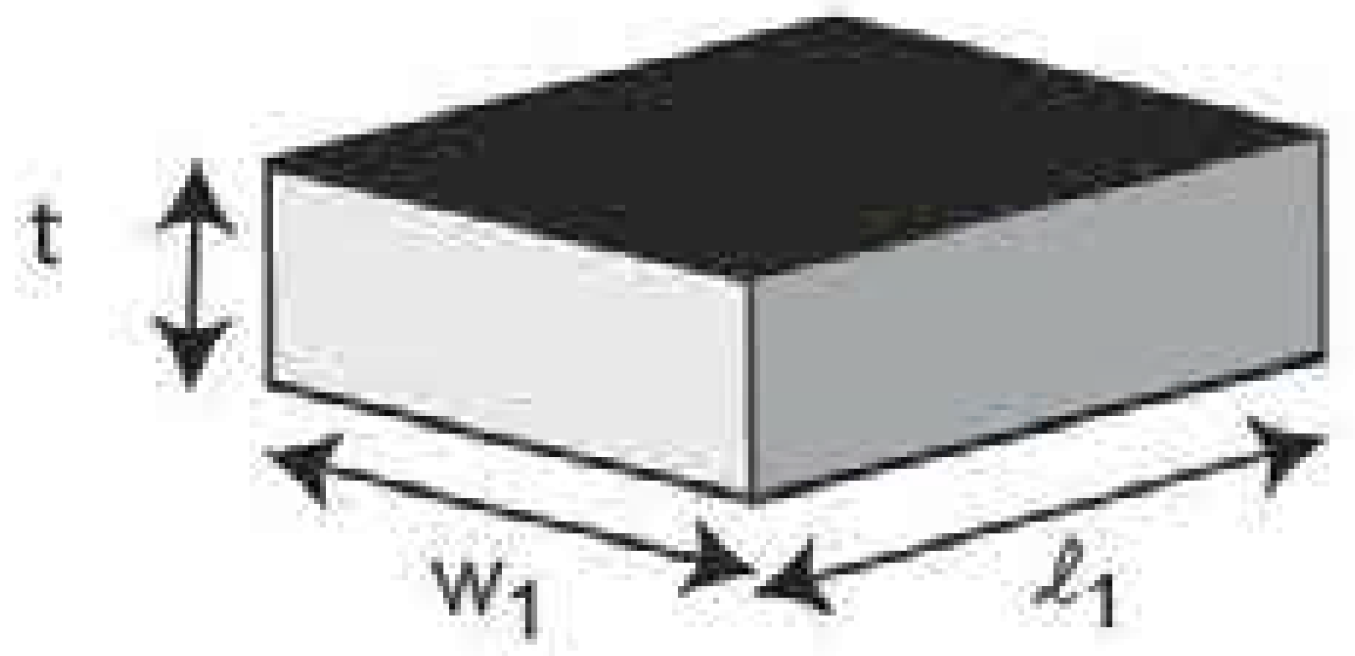
\includegraphics[width=0.2\textwidth]{images/ResistivityGeometry.png}
			\caption{Resistivity Geometry}
			\label{Fig:ResGeometry}
		\end{figure}
		The resistance between two opposite edges of a rectangular volume having width $w$, length $l$ and height $t$ is given by: 
		\begin{equation}
			R = \rho \cdot \frac{l}{A} = \rho \cdot \frac{l}{t\cdot w}
		\end{equation}
		with 
		\begin{itemize}
			\setlength{\itemsep}{-5pt}
			\item[] \makebox[1.5em][l]{$dl$} = Change in length of the material in the direction being measured
			\item[] \makebox[1.5em][l]{$l$} = Overall length of material in the direction being measured
			\item[] \makebox[1.5em][l]{$dT$} = Change in temperature over which $dl$ is measured
		\end{itemize}
		If $l = w $ , the resistance becomes $R = \frac{\rho}{l}$ which is referenced as the \textbf{surface resistivity $\sigma$}. 
	\subsection{Dielectric Strength and Breakdown}
		The dielectric strength of a material is the ability to resist the passage of a disruptive discharge produced by an electric stress, this values do depend on the environment. 
		\begin{itemize}
			\setlength{\itemsep}{-5pt}
			\item[] FR-2 $\rightarrow$ 29 MV/m
			\item[] FR-4 $\rightarrow$ 20 MV/m
		\end{itemize}
		\begin{table}[h!]
			\centering
			\begin{tabular}{|m{0.2\textwidth}|m{0.2\textwidth}|m{0.2\textwidth}|m{0.2\textwidth}|}
				\hline
					\textbf{DC (peak AC) voltage between conductors} & \textbf{Minimum Spacing (sea level to 3km) uncoated board} & \textbf{Minimum Spacing (above 3km)} & \textbf{Minimum Spacing conformal board}\\
				\hline
				\hline
					50 V & 0.63 mm & 0.63 mm & 0.38 mm  \\
				\hline
					500 V & 2.54 mm & 12.7 mm & 1.51 mm  \\
				\hline
					$>$ 500 V & 0.051 mm/V & 0.127 mm/V & 0.03 mm/V \\
				\hline
			\end{tabular}
			\caption{Recommended conductor spacing}
			\label{Tab:ConductorSpacing}
		\end{table}
		
	\subsection{Loss Angle}
		The dielectric strength of a material is the ability to resist the passage of a disruptive discharge produced by an electric stress, this values do depend on the environment. 

		\begin{table}[h!]
			\centering
			\begin{tabular}{|m{0.2\textwidth}|m{0.2\textwidth}|m{0.2\textwidth}|m{0.2\textwidth}|}
				\hline
					\textbf{Material} & \textbf{$\varepsilon_r$} & \textbf{tan $\delta$} & \textbf{MV/m}\\
				\hline
				\hline
					Air & 1.0006 & 0  & 3  \\
				\hline
					Polycarbonate & 2.3 & 0.0012 & 275  \\
				\hline
					FR-4 & 4.4 & 0.035 & 70 \\
				\hline
					Alumina & 8.8 & 0.00033 & 12 \\
				\hline
					Barium Titanate & 1200+ & 0.01 & 2 \\
				\hline
			\end{tabular}
			\caption{Loss angle and break voltage for different material @ 1MHz}
			\label{Tab:LossAngle}
		\end{table}
		\begin{table}[h!]
			\centering
			\begin{tabular}{|m{0.2\textwidth}|m{0.2\textwidth}|m{0.2\textwidth}|}
				\hline
				\textbf{Frequency} &	\textbf{$\varepsilon_r$} & \textbf{tan $\delta$}\\
				\hline
				\hline
					 100 Hz	& 4.80& 0.009\\
				\hline
					 1 kHz	& 4.75& 0.012\\
				\hline
					 10 kHz	& 4.70& 0.015\\
				\hline
					 100 kHz& 4.65& 0.018\\
				\hline
					 1 MHz	& 4.60& 0.020\\
				\hline
					 10 MHz	& 4.55& 0.022\\
				\hline
					 100 MHz& 4.50& 0.024\\
				\hline
					 1 GHz  & 4.45& 0.025\\
				\hline
					 10 GHz & 4.40& 0.025\\		
				\hline			 
			\end{tabular}
			\caption{Dielectric Constant $\varepsilon_r$ and dissipation factor $tan \delta$ for FR-4}
			\label{Tab:LossAngleFR4}
		\end{table}
		
		
		\begin{table}[h!]
		\centering
		\begin{tabular}{|m{0.165\textwidth}|m{0.35\textwidth}|m{0.415\textwidth}|}
		\hline
			
				\textbf{Expansion Type} & &\\
		\hline
		\hline
				Flexural Strength
			& 
				 \begin{center}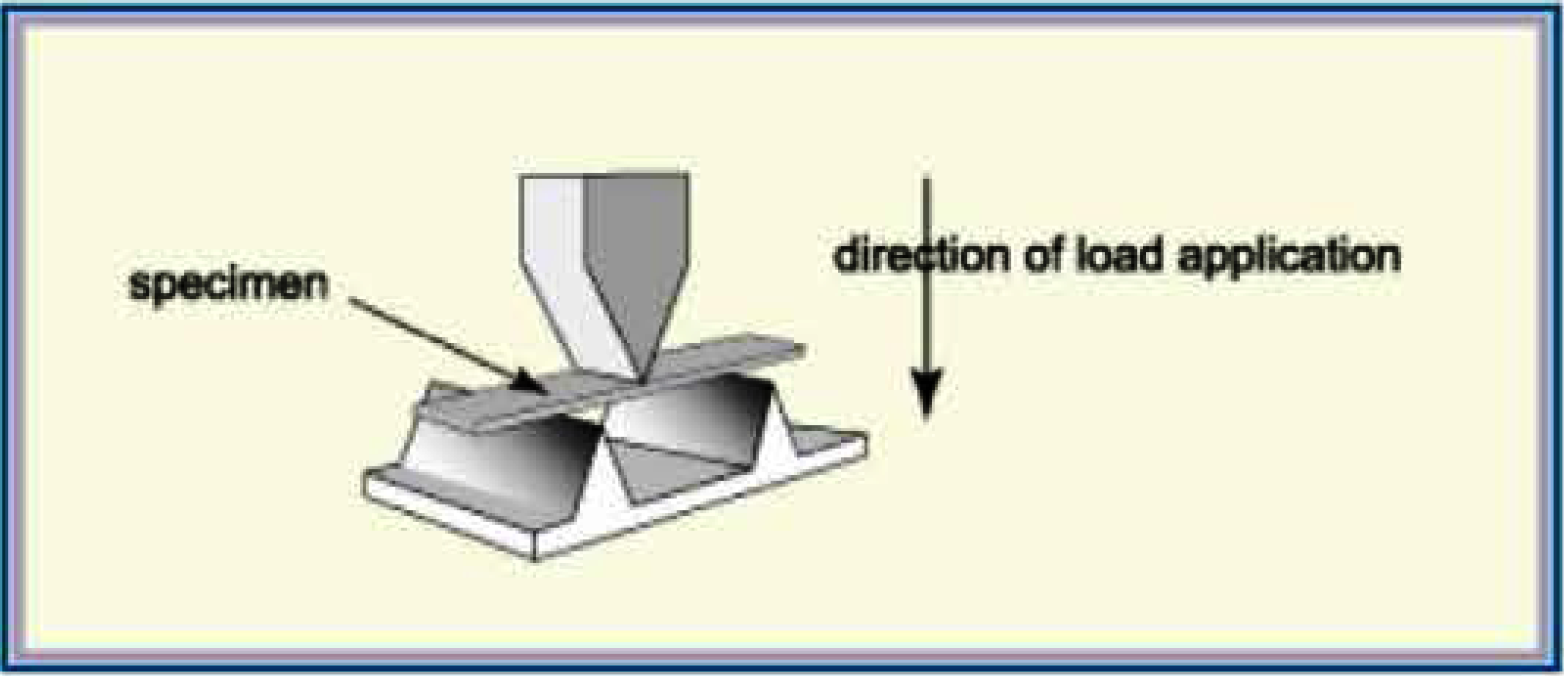
\includegraphics[width=0.35\textwidth]{images/FlexuralStrength.png}\end{center}  
			&
				For materials that do not break, the flexural strength is usually reported as the load at which 5\% deformation of the outer surface occurs. Both flexural strength and flexural modulus will be functions of temperature, with their values reducing with increased temperature, even below glass transition. \newline Example: \newline FR2 (lengthwise) = 83 MPa \newline FR2 (crosswise) = 72 MPa \newline FR4 (lengthwise) = 414 MPa \newline FR4 (crosswise) = 345 MPa
			\\
		\hline
				Stiffness
			& 
				 \begin{center}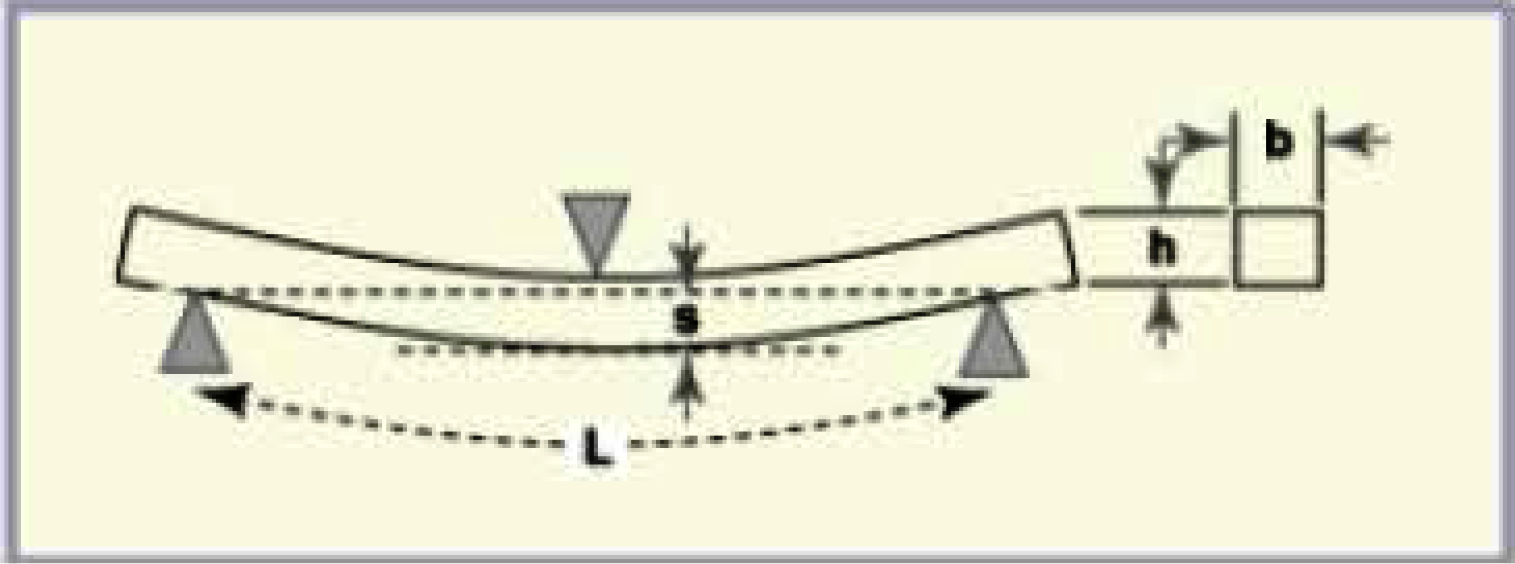
\includegraphics[width=0.35\textwidth]{images/Stiffness.png}\end{center}  
			&
				\begin{equation}
					\sigma_f = \frac{3FL}{2bh^2}
				\end{equation}
				\begin{equation}
					s = \frac{\varepsilon_f L^2}{6h}
				\end{equation}
				\begin{equation}
					E = \frac{\sigma_{f2}-\sigma_{f1}}{\varepsilon_{f2} - \varepsilon_{f1}}
				\end{equation}
				with\newline
				F = Load applied at centre of beam [N]\newline
				L = Distance between support points [mm]\newline
				b = Width of beam [mm] \newline
				h = Thickness of beam [mm]\newline
				s = Deflection at centre of beam [mm]\newline
				$\sigma_f$ = Flexural stress [MPa]\newline
				$\varepsilon_f$ = Inner Strain (Dehnung) per unit length in \% \newline
				Suggested strains for linear behaviour = 0.5 \% and 2\%
			\\
		\hline
				Bow and Twist
			& 
				 \begin{center}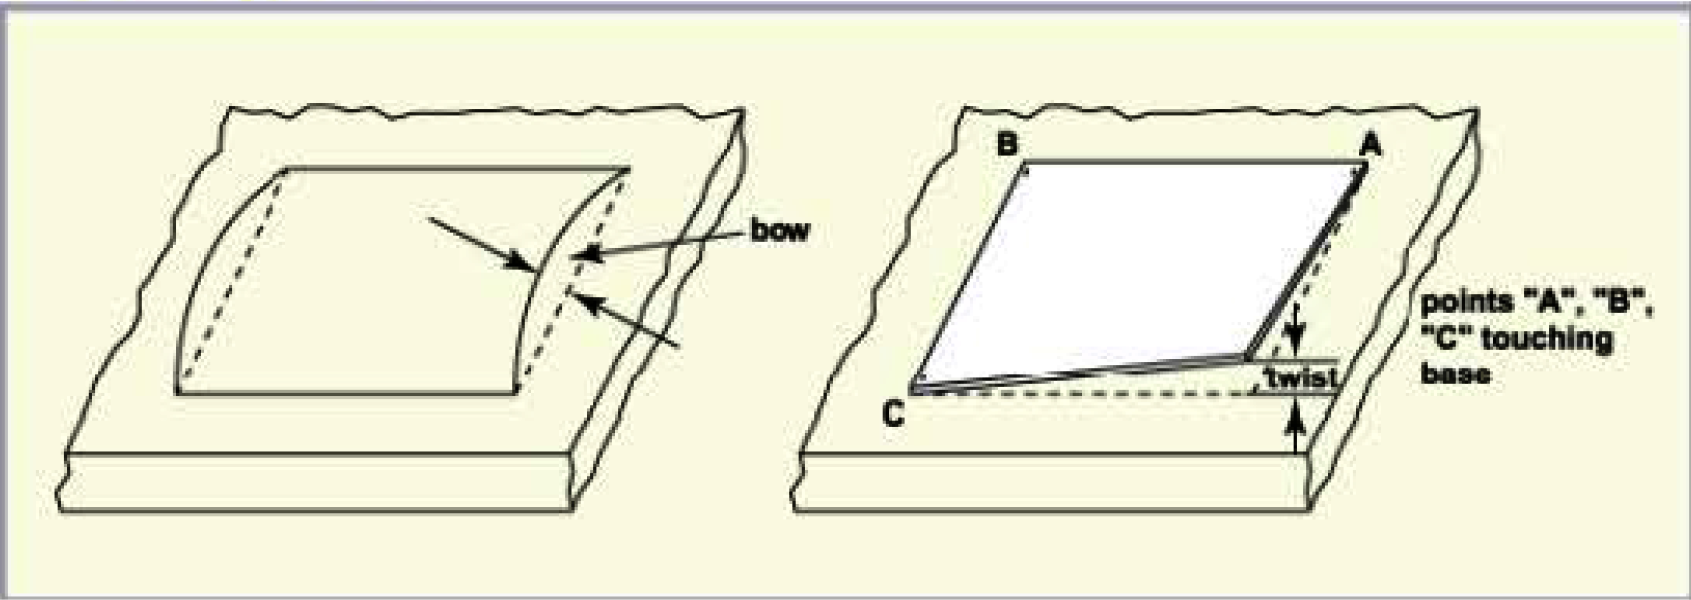
\includegraphics[width=0.35\textwidth]{images/BowTwist.png}\end{center}  
			&
				\textbf{Bow}\newline
				Is characterised by a cylindrical curvature of the board, so that all four corners are in the same plane, bu the centre is raised. \newline
				\textbf{Twist}\newline
				Is the deformation parallel to a diagonal, so that only three of the four corners of a rectangular sheet lie in the same plane. 
			\\
		\hline
		\end{tabular}
		
		\caption{Expansion Types}
		\label{Tab:ExpansionTypes}
		\end{table}
	\subsection{Layer Builds, Layout Rules, Flex circuit, Vias, Sequential Build up Layers (SBU), Any Layer interstitial via holes (ALIVH), Standards}
	See lecture slides. 
\newpage